\section{Auswertung}
\label{sec:Auswertung}

\subsection{Bestimmung des Schubmoduls ohne Magnetfeld}
Das Gesamtträgheitsmoment $\theta_\text{ges}$ ergibt sich aus der Summe des Trägheitsmomentes
der Kugel $\theta_\text{Kugel}$ nach Gleichung (11), und dem gegebenen Trägheitsmoment der Halterung $\theta_\text{h}$ zu
\begin{align*}
  \theta_\text{ges} = {} & \theta_\text{Kugel} + \theta_\text{h} \\
                    = {} & (1,53 \cdot 10^{-4} \pm 1,4 \cdot 10^{-7})\,\si{\kilo\gram\meter\squared} + 2,25 \cdot 10^{-6}\,\si{\kilo\gram\meter\squared} \\
                    = {} & (1,5525 \cdot 10^{-4} \pm 1,4 \cdot 10^{-7})\,\si{\kilo\gram\meter\squared}.
\end{align*}

\noindent Zur Bestimmung des Schubmoduls $G$ werden nun 10 Schwingungsperioden ohne Magnetfeld $B$ gemessen (Tabelle 1).


\begin{table}[H]
\centering
\caption{Periodendauer $T$ des zur Schwingung angeregten Drahtes ohne Magnetfeld $B$.}
\label{tab:ohnebfeld}
\begin{tabular}{c c}
\toprule
Fehler & T\:/\:s\\
\midrule
 & 18,247 \\
 & 18,242 \\
 & 18,244 \\
 & 18,245 \\
 & 18,250 \\
 & 18,249 \\
 & 18,243 \\
 & 18,235 \\
 & 18,248 \\
 & 18,250 \\
\hline
Mittelwert & 18,245 \\
Standardabweichung & 0,004 \\
\bottomrule
\end{tabular}
\end{table}

\noindent Mit der Länge $L$ und dem Durchmesser $d$ des Drahtes (Tabelle 2) lässt sich nach Gleichung (12) den Schubmodul $G$ zu 

\begin{table}
\centering
\caption{Messgrößen des Drahtes.}
\label{tab:ohnebfeld}
\begin{tabular}{c c c}
\toprule
 & d\:/\:mm & L\:/\:cm\\
\midrule
 & 0,172 & 66,30 \\
 & 0,173 &  \\
 & 0,170 & \\
\hline
Mittelwert & 0,172 & \\
Standardabweichung & 0,001 & \\
\bottomrule
\end{tabular}
\end{table}

\begin{align*}
G = (1,41 \pm 0,04) \cdot 10^{11}\,\si{\newton\per\meter\squared}
\end{align*}
berechnen.\\~\\

\noindent Der Elastizitätsmodul $E$ wird aufgrund der fehlenden experimentellen Bestimmung nach Literaturwerten
\begin{align*}
E = 210\,\si{\giga\pascal}
\end{align*}
gesetzt.
\\~\\
\noindent Nach Gleichung (3) ergibt sich für die Poissonsche Querkontraktionszahl
\begin{align*}
\mu = {} & \frac{E}{2G} - 1 \\
    = {} & (0,257 \pm 0,022)
\end{align*}

\noindent und daraus über die Gleichung (4) für den Kompressionsmodul
\begin{align*}
Q = {} & \frac{E}{3(1-2\mu)}\\
  = {} & (1,44 \pm 0,13) \cdot 10^{11}\,\si{\pascal} .
\end{align*}

\subsection{Bestimmung des magnetischen Momentes eines Permanentmagneten}
Die Magnetfeldstärke $B$ im Zentrum des Helmholtz-Spulenpaars ergibt sich zu
\begin{align*}
B_\text{H} = \mu_0 \frac{8NI}{\sqrt{125} R }
\end{align*}
mit $N=80$ und $R=72\,\si{\milli\meter}$.

\begin{table}
\centering
\caption{Periodendauer $T_\text{m}$ des zur Schwingung angeregten Drahtes mit eingeschaltetem Magnetfeld $B$.}
\label{tab:periodendauer}
\begin{tabular}{c c c c c c}
\toprule
\multicolumn{1}{c}{Stromstärke} & & & $T_\text{m}\:/\:\si{\second}$ & & \\
{$I\:/\:\si{\ampere}$} & {0,4} & {0,5} & {0,6} & {0,8} & {1} \\
\midrule
 & 5,670 & 5,087 & 4,576 & 3,842 & 3,301\\
 & 5,687 & 5,039 & 4,596 & 3,856 & 3,284\\
 & 5,659 & 5,046 & 4,611 & 3,846 & 3,276\\
 & 5,682 & 5,090 & 4,603 & 3,847 & 3,270\\
 & 5,441 & 5,107 & 4,597 & 3,831 & 3,289\\
\hline
Mittelwert & 5,6278 & 5,0738 & 4,5966 & 3,8444 & 3,2840 \\
St.Abw. & 0,0939 & 0,0265 & 0,0116 & 0,0081 & 0,0107 \\
\hline
Magnetfeld $B\:/\:\si{\milli\tesla}$ & 0.3996 & 0.4995 & 0.5995 & 0.7993 & 0.9991\\
\bottomrule
\end{tabular}
\end{table}

\noindent Nach Umstellen der Gleichung (17) erhält man
\begin{align}
\Psi := m_\text{mgn}B + D = \frac{4\pi^2\theta_\text{ges}}{T_\text{m}^2}.
\end{align}

\noindent Um das magnetische Moment $m_\text{mgn}$ zu berechnen wird nun $\Psi$ gegen
die Magnetfeldstärke $B$ aufgetragen (Abbildung 6) und mithilfe linearer Regression 
wird die Steigung der Ausgleichsgeraden bestimmt:

\begin{align*}
m_\text{mgn} = (0,628 \pm 0,035)\,\si{\ampere\meter\squared}\\
D = (-7,3 \pm -2,4) \cdot 10^{-5}\,\si{\kilo\gram\meter\squared\per\second\squared}.
\end{align*}

\begin{figure}[H]
 \centering
  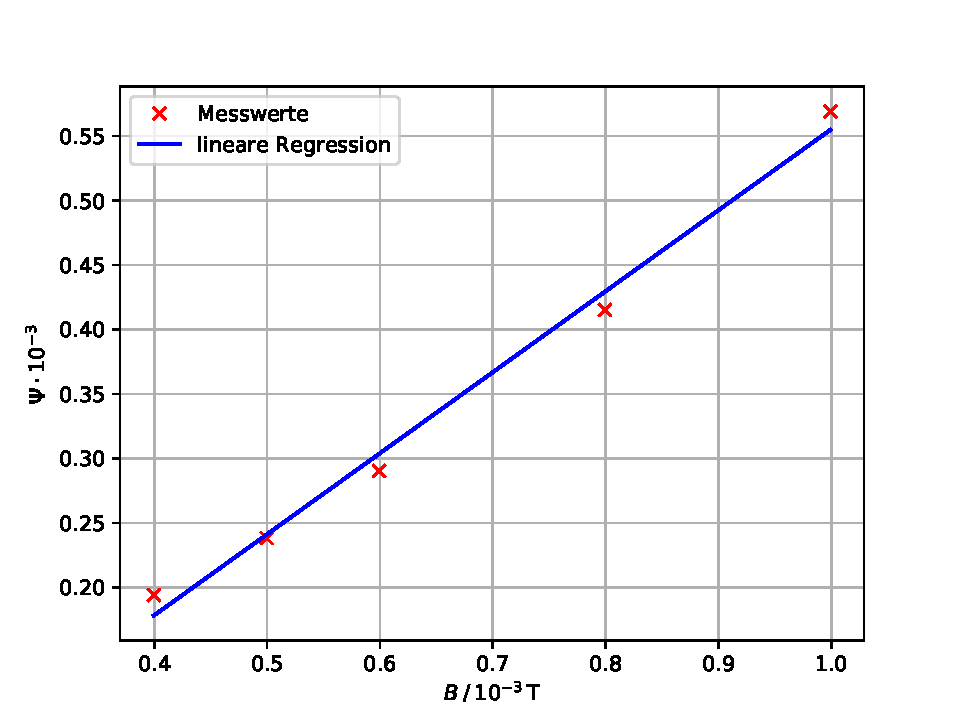
\includegraphics{linreg.pdf}
  \caption{$\Psi$-$B$-Diagramm und lineare Regression}
  \label{fig:drill}
\end{figure}